\chapter{Développement durable}

A l'heure où la France s'inquietait de l'impact des climatiseurs pour refroidir nos pièce sur la planète, la Malaisie, et notament UTP ne semblent par encore être préoccupé par ce problème.

Les températures extérieures étant très élevées en Malaisie, tous les batiments (gare, restaurants, hotels, etc.) et les voitures sont équipés de climatiseurs. Cependant le réglages de ces derniers sont souvent bien trop froid ($< 20^{\circ}C$) et nous oblige à porter des vetements chauds et long à l'interieur des batiments, malgré la temparature dépassant largement les $30^{\circ}C$ à l'éxterieur sur l'ensemble de  notre séjour.

\begin{figure}[h]
  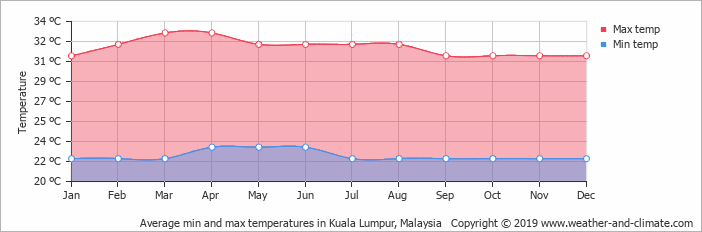
\includegraphics[width=1\linewidth]{content/imgs/temp.png}
  \caption{Temperatures moyennes minimales et maximales en Malaisie, dans la capitale}
  \label{fig:climate}
\end{figure}

Malgré l'usage excessifs des climatiseurs, les batiments récents de l'université ne sont en général pas dotés d'une isolation thermique comparable aux batiments récents construit en France. Pour ne prendre qu'un exemple, je travaillais dans la bibliothèque universitaire, cette dernière possède une immense façade vitrée bordée de porte, elles aussi vitrées, tout le long laissant la fraicheur du batiments se faire ressentir sur plusieurs mètre à l'exterieur.

D'après le site de l'université \cite{utp_gender}, une attention particulière est mise en oeuvre pour favoriser la diversité des genres au sein de l'université, que ce soit au niveau des étudiants, des employés et du personnel pédagogique.
